\documentclass[]{usiinfbachelorproject}
\usepackage{graphicx}
\usepackage{placeins}
\usepackage{float}
\usepackage{subfigure}
\usepackage{listings}
\usepackage{multicol}

% Settings for code listings
\lstset{
  basicstyle=\ttfamily, % Use small monospace font
  columns=flexible,
  breaklines=true,
  frame=single,
  xleftmargin=2pt,
  xrightmargin=2pt,
}
\captionsetup{labelfont={bf}}

\author{Hun Rim}

\title{Time Series Forecasting of European Energy Market}
\subtitle{European Market and Renewables}
\versiondate{\today}

\begin{committee}
%With more than 1 advisor an error is raised...: only 1 advisor is allowed!
\advisor[Universit\`a della Svizzera Italiana, Switzerland]{Prof.}{Olaf}{Schenk}
%You can comment out  these lines if you don't have any assistant
\assistant[Universit\`a della Svizzera Italiana, Switzerland]{Title}{Juraj}{Kardos}
\end{committee}

\abstract {
The ambitious energy targets, accelerated by the recent energy crisis, are driving the European Union to increase the share of renewable energy in gross energy consumption to 42.5\% by 2030 from the current 23\%. However, the intermittent and seasonal nature of renewable energy sources presents challenges in predicting their production capacity. The ability to accurately forecast the evolution of renewable energy’s stake in the dynamic and ever-evolving energy market is a critical component in the decision making process of policy makers, and market participants alike. This project aims to explore and evaluate the performance of well-established forecasting methods in anticipating the trends of individual renewable energy components, ultimately contributing to the fostering of a balanced, sustainable, and reliable energy market in the EU. 
The primary focus is to assess auto-regressive forecasting methods and advanced models incorporating moving-average, exploit seasonality of time series data, or those utilising the correlation with exogenous variables. The results are presented for data considering recent history of the most significant enegy component at the European energy markets.
}


\begin{document}
\maketitle

%%%%%%%%%%%%%%%%%%%%%%%%%
\section{Introduction} \label{introduction}
%%%%%%%%%%%%%%%%%%%%%%%%%

Like a staple good, we have steady demand for energy in our daily lives unlike luxury goods, and this demand is growing everyday due to increase in gross energy consumption per capita, advancement of technology, and increase in population. Furthermore, non-renewable energy, which is still a dominant source of energy, and its' production is a major source of global warming. As a result, the European Union set multi-stage goals to reach 100\% reliance on renewable energy in upcoming decades. However, the production of renewable energy sources like solar or wind power often faces challenges due to their intermittent nature, influenced by factors such as climate conditions. Consequently, market participants in European energy market encounter difficulties in effectively balancing the fluctuating supply and demand of energy in this dynamic and transitioning market environment.   \\ 

Policymakers and other energy market participants often stress that they need the grid operational statistics faster, particularly the European energy supply including renewable energy components, and consumption. When visualized, monthly energy demand reveals distinct patterns, with cyclical peaks occurring during winter and lows in summer, notably in July and August. These observations not only highlight Europe's heightened energy consumption in colder seasons, but also prove the data's seasonality. Suggesting the possibility of translating these patterns into mathematical models which can allow forecasting of future values. The goal of the project is to develop a framework for forecasting the individual energy components contributing to the overall energy balance in Europe. The framework consists of well-established forecasting methods which can be easily applied to the energy market data, and auxiliary methods which compare the forecast of various methods and statistically evaluate the method's reliability. \\

\subsection{Auto-Regressive Integrated Moving-Average}
ARIMA model is one of the most widely used statistical forecasting model. It is a generalized version of AutoRegressive Moving-Average (ARMA) model and difference between the two models is their ability to handle non-stationary data. Stationarity indicates constancy of statistical property of a dataset such as variance, or mean over time. When data is stationary, it guarantees the stability of underlying patterns in the dataset, and eradicates the concern of the pattern being a result of random fluctuation. ARIMA model is capable of adjusting the data to provide this stability unlike ARMA. \\

Autoregression is a technique used in time series analysis that assumes temporal trend between the values in the dataset, and uncover a function of order \textit{p}. In the auto-regression model, the variable regresses against itself. Put simply, the current value is calculated from previous values, by estimating the influence of these past values on the present value under the assumption there is a temporal dependency between the values of the variable. However, even if we assume the general trend is captured perfectly, there are inconsistent white-noise in the data which are not replicable. ARIMA model utilizes Moving-average component to estimate the white-noise in the data by studying the temporally closest known white-noises, and capture the short-term fluctuations which are not reflected by only studying the general trend. All these factors are combined to formularize ARIMA model (${ARIMA(p, d, q)}$) as the following: \\

\begin{equation}
    ARIMA(p,d,q) = C + \sum_{i=1}^{p} \psi_i L_{N - i}^{(d)} + \sum_{j=1}^{q}\varphi_j\epsilon_{N-j} + \epsilon_{N}
\end{equation}

If we dissect the equation we can observe ${\epsilon_N}$, this denotes the unknown error between the forecasted value and the actual value. Signifying, regardless of how well the model fits the data, there will be some uncertainty in the forecast.

\subsection {Seasonal ARIMA}

As mentioned, the EU energy market data often exhibits seasonal patterns. Seasonal-ARIMA model is an extension of the standard ARIMA model which incorporates the seasonal component, and specifically handles seasonal patterns of the time series data when making a forecast. Essentially, this model does not stop at reflecting lags but extends to reflects on same period of previous years to certain degree if there is an annual periodicity. Similar to the representation of the ARIMA model, SARIMA model is denoted as ${ARIMA(p,d,q)(P,D,Q)_m}$, and can be formularized as the following: \\ 

\begin{equation}
    ARIMA(p,d,q)(P,D,Q)_m = ARIMA(p,d,q) + \sum_{i=1}^{P}\Phi_i L_{N - im}^{D} + \sum_{j=1}^{Q}\Theta_j \epsilon_{N - jm}  
\end{equation} 

Just as ${(p, d, q)}$ represents the order of autoregression,
integration, and moving-average, ${(P, D, Q)_m}$ represents the components but in a seasonal scale. The ${m}$ denotes length of season, which in our case will be 12 months. \\

\subsection{Exogenous Variables}

The EU power sector, just like any other power sector, experiences
volatility due to external factors such as the climate. No matter how
accurate the ARIMA model is at forecasting, it has no bypass to
account for the forecast errors originating from external factors,
and this also applies to SARIMA model. Hence, the framework consists of a statistical model extending the ARIMA called SARIMAX
(SARIMA with eXogenous variables) which also is capable of accounting for both seasonality, and errors due to the external factors. In this model, the external variable which has influence on the European power sector such as the economic or climate indicators
can be factored in to the appropriate time frame. When forecasting
the market movements, instead of soley relying on temporal correlation and statistical factors, the SARIMAX model can additionally reflect on the previous time frames with similar exogenous indicators to produce a better forecast. \\

\begin{equation}
    SARIMAX(p,d,q)(P,D,Q)_m = ARIMA(p,d,q)(P,D,Q)_m + \sum_{i=1}^{k}\beta_i Z_{i}
\end{equation} 

As it can be seen in the equation above, the SARIMAX model is built on SARIMA model with additionally accounting for ${k}$ exogenous variables. \\

\subsection{Deep-Learning with Recurrent Neural Network}
Along with predictive statistics, deep learning (DL) is frequently used in forecasting. Especially, deep learning model using Recurrent-Neural-Network (RNN) with Long Short-term Memory (LSTM) layers, as shown in figure ~\ref{fig:lstm}, is very popular with time series forecasting. RNN iteratively repeats the process of aggregation and activation unlike normal neural networks, and LSTM extends the memory of RNNs to allow the capturing of long-term dependencies. This regression like property of RNN, and the reinforcement of its capability from LSTM layer makes it very effective when building a time series forecasting model. Furthermore, it would be fascinating to make a comparison between the performance of various predictive statistical model, and a deep-learning model. \\

\begin{figure}[htp]
    \centering
    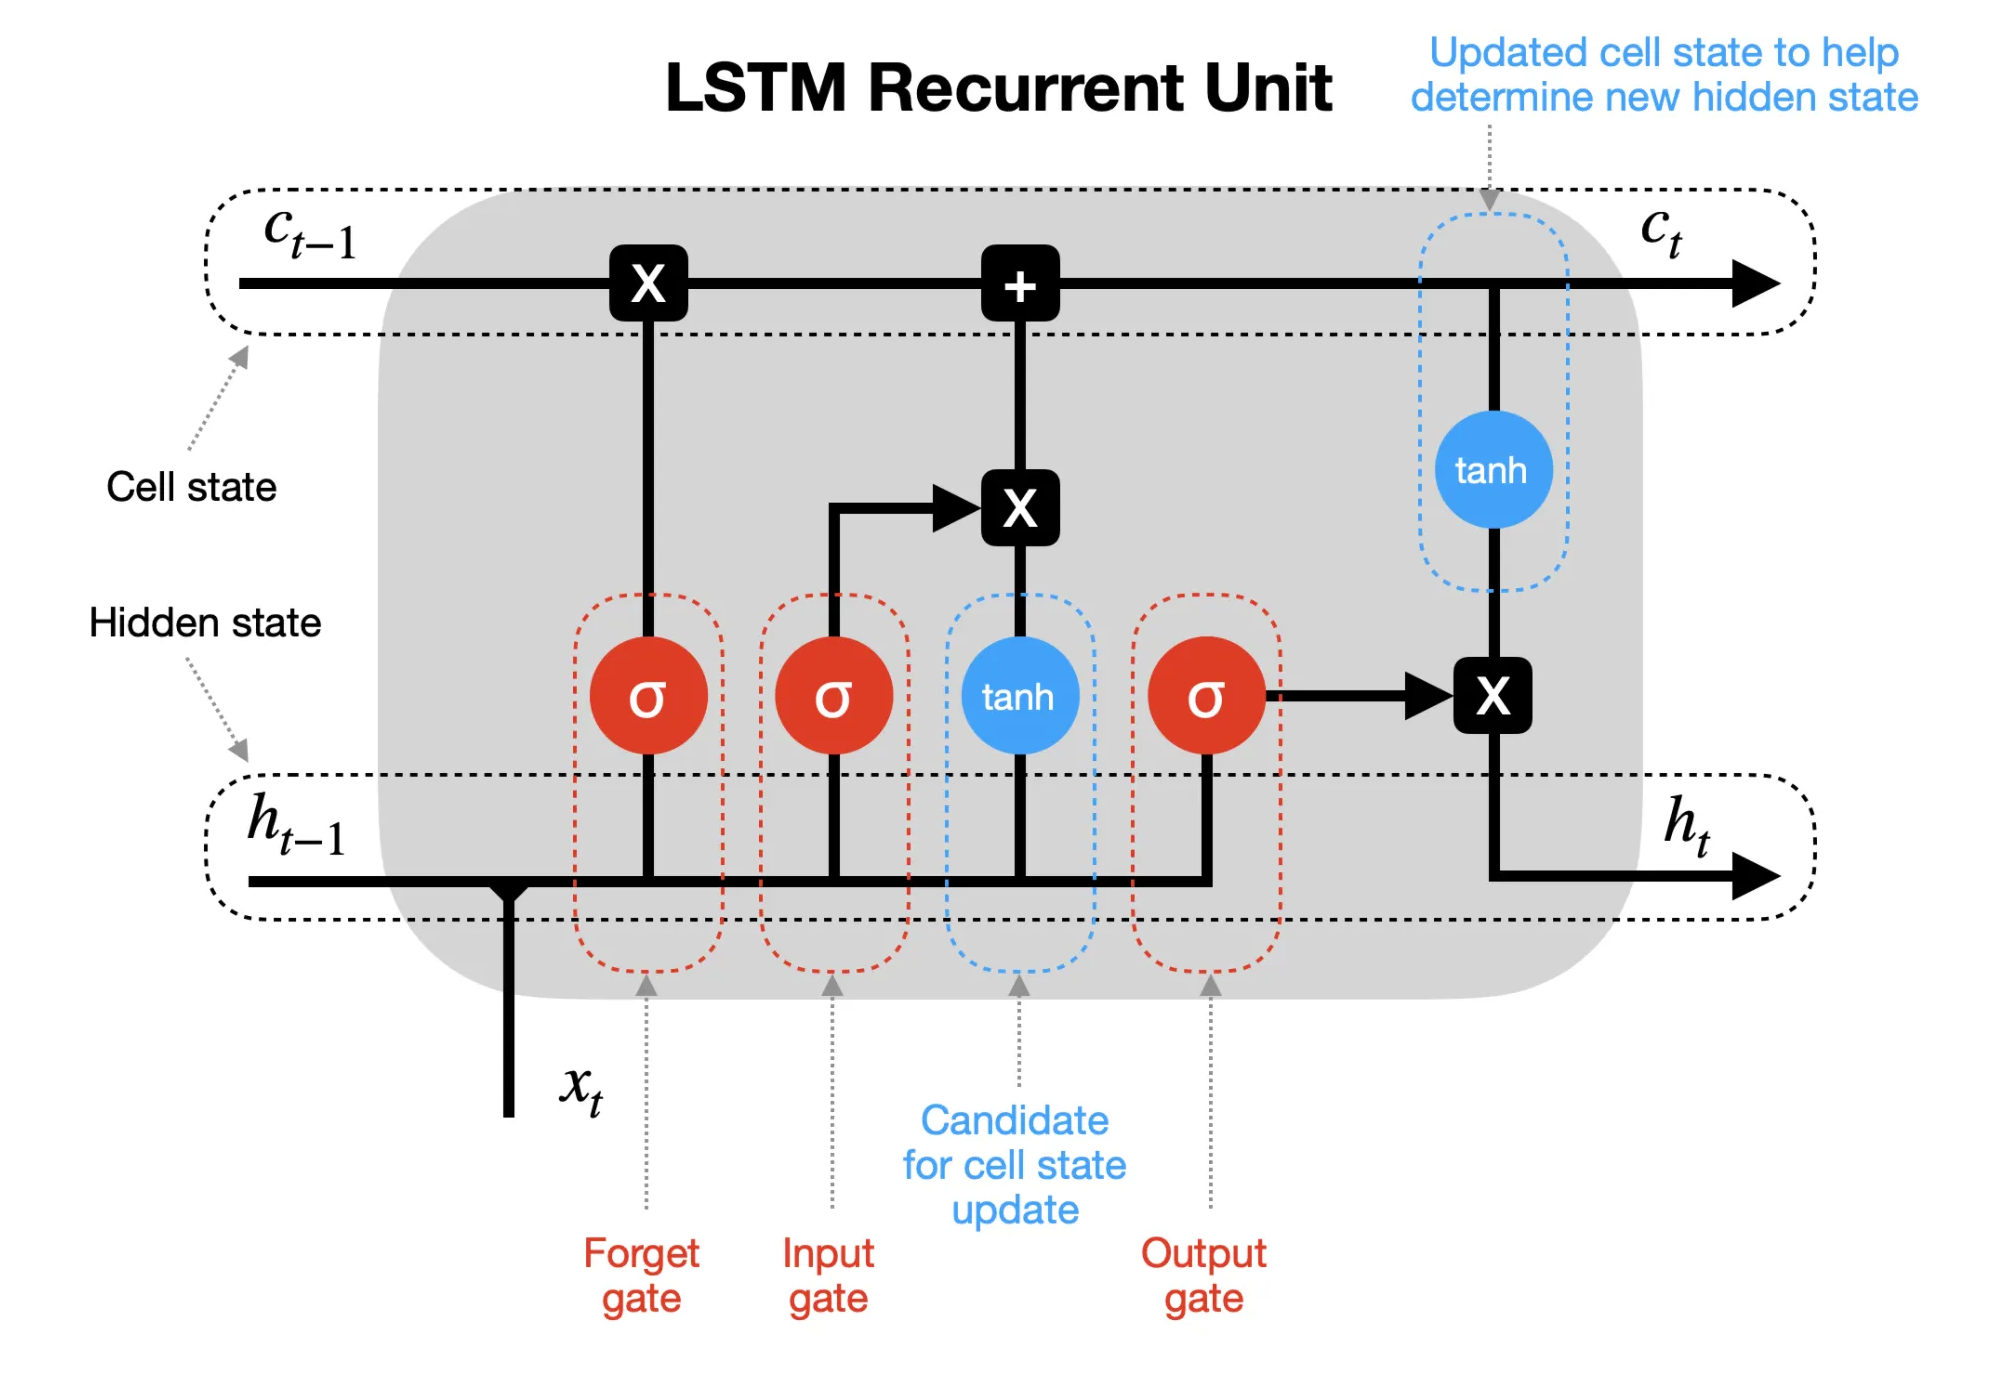
\includegraphics[width=0.6\linewidth]{figures/lstm.png}
    \caption{Structure of LSTM Recurrent Unit}
    \label{fig:lstm} % Tag for referencing
\end{figure}

\section{Experimental Setup}
This sections presents the setup of the development environment and forecasting methods considering the study and presents the data that will be used to evaluate the forecasting accuracy.\\

\subsection{Developer Environment}
\begin{itemize}
 \item System Environment: Linux Ubuntu 20.04.06 LTS
 \item Environment Manager: Anaconda (conda 23.9.0)
 \item Programming Language: Python 3.9.15
 \item Python Libraries: 
 \begin{itemize}
    \item pandas: 1.5.3
    \item numpy: 1.26.0
    \item statsmodel: 0.14.0
    \item pmdarima: 2.0.4
 \end{itemize}
\end{itemize}

\subsection{Parametrization of Statistical Methods}
The autoregressive models need to be parametrized by a set of parameters ${(p, d, q)}$. There are mainly 2 approaches in deriving the ${(p,d,q)}$ values, and first method is calculating the $d$ value through differencing the dataset until the result of Augumented Dickey-Fuller test falls below 0.05 and disproves the Null-Hypothesis.
Then, finding the order of autoregression $p$ through the decay
of AutoCorrelation Function (ACF), and finding the order of moving-average $q$ through the decay of Partial-Auto Correlation Function (PACF). Second approach is using a brute force approach such as $Grid-Search$. Grid search algorithm finds the minimum Akaike Information Criterion (AIC) value by iterating through a fixed range of parameters of different order. Naturally, first method is more efficient whereas the second method is computationally inefficient but more simple to implement. However, as computational complexity problem is becoming negligent due to the significant enhancement of computational power. In our framework, orders are determined by \textit{auto\_arima()} function of Python, a built-in search algorithm from \textit{pmdarima} library with the grid search elements. It is important to note that depending on the passed parameters, the resultant order and seasonal order differs drastically. \\

\begin{figure}[htp!]
    \begin{lstlisting}[language=Python]
    stepwise = auto_arima(
        data, exogenous=exo_train, m=period, seasonal=m, stepwise=True,
        test="adf", information_criterion="aic", method="nm", maxiter=100,
        start_p=0, start_q=0, start_d=0, max_p=5, max_q=2, max_d=5, 
        start_P=0, start_Q=0, start_D=0, max_P=5, max_Q=2, max_D=5, 
    )
    order = stepwise.order
    seasonal_order = stepwise.seasonal_order
    \end{lstlisting}
    \caption{Configuration of auto\_arima() function}
    \label{fig:autoarimaconfig}
\end{figure}

While some values of the parameters are common for all methods, some differ depending on the method.

\subsubsection{Common parameters of auto\_arima()}
\begin{itemize}
\item X, y: In our case, the X, and y is contained in the variable "data", which is a pandas dataframe with DateTimeIndex as the index (x-axis), and corresponding quantity of a specific energy (y-axis) in a EU country at the index month. \\

\item test: This is a parameter indicating which statistical test, the Augumented-Dickey-Fuller test in our example, to utilize while checking for stationarity during the search for the order of ARIMA or SARIMA functions. \\

\item stepwise: This particular parameter indicates whether the algorithm should do a full grid search (if False), an exhaustive search method or perform a more efficient search (if True) through an optimization method. \\

\item method: The parameter "method" refers to optimization method used for the search of the parameters when the stepwise parameter is "True". This parameter holds significant importance in calculating the correct order parameter as depending on the search algorithm, the accuracy can differ drastically.\\

The auto\_arima function has multiple built-in optimization method, and calls \textbf{Limited-memory Broyden-Fletcher-Goldfarb-Shanno} (l-bfgs) method in default, which is a practical gradient-based optimization method for large dataset due to its' quick convergence and memory efficiency. However, l-bfgs and other gradient-based search methods have a common problem of requiring a scenario-specific delicate tuning of hyperparameters. This is because both methods rely on line search to determine appropriate step-size in a search direction to sufficiently decrease the objective function. When hyperparameters such as initial stepsize are poorly tuned, it leads to inefficient searches or convergence issues. Furthermore, gradient-based methods typically perform poorly in noisy, non-differentiable data. As it can be seen in figure ~\ref{fig:france_wind}, our data is non-differentiable, and if we view the Resid (measurement of residuals in the data), it is quite noisy as well. \\

As a result, the \textit{Nelder-Mead} (nm) optimization method was chosen for the search. Nelder-Mead optimization method specifically performs well on data which are generally noisy and non-differentiable as it is gradient free. Naturally, it performed significantly better than gradient-based methods in finding the optimal order parameters from our data which has exactly those characteristics. In addition, it proved to be consistent, flexible, and robust in working with data from various energy sources of various countries. Biggest constraint of Nelder-Mead is that it performs poorly on large-scale data. However, as our data has long temporal interval between the adjacent values, we would not need to worry about our dataset being too large. Hence, it was the perfect optimization method for our framework.\\

\begin{figure}[htp!]
    \centering
    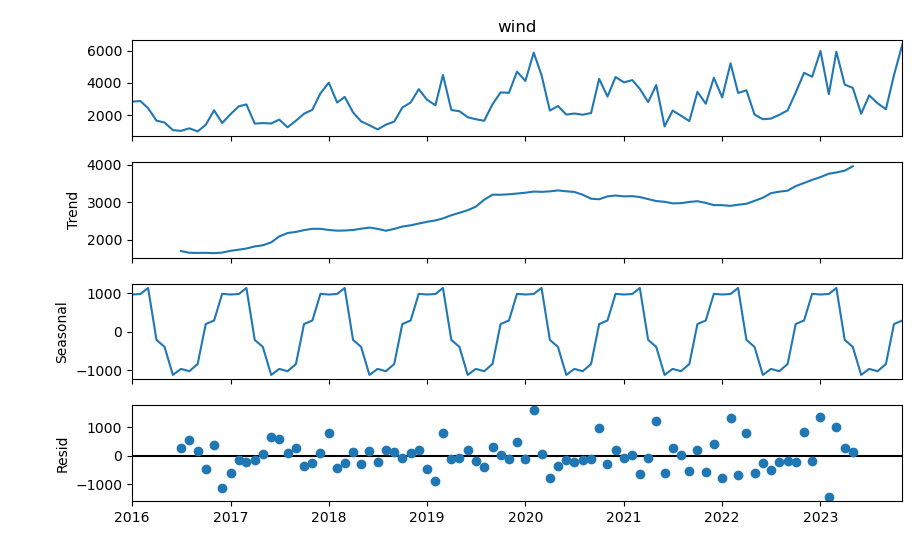
\includegraphics[width=0.5\linewidth]{figures/France_wind.png}
    \caption{Seasonal Decomposition of Wind Energy Production in France}
    \label{fig:france_wind} % Tag for referencing
\end{figure}

\item maxiter: This parameter sets the maximum number of iterations for the optimization method to find the convergence. The default maximum number of iteration for optimization method is 50 but our framework allows upto 100 iterations to accommodate for complex functions, which is quite common in our data. \\

\item start and max (p, d, q): By setting the range for order parameters the framework avoids doing an exhaustive search or missing the optimal parameter values due to lacking range for exploration. In this case, $p$ and $q$ are set between 0 and 5, while setting the differential order between 0 and 2. \\

\item information\_criterion: Information Criterion refers to statistical measures used for model selection, and it is crucial in selecting optimal order parameters for the model. Conventionally, there are 2 commonly used information criterions which are Akaike (AIC) and Bayesian (BIC). As it can be seen in figure ~\ref{fig:autoarimaconfig}, the AIC is chosen.\\

\newpage
\begin{equation}
    AIC = 2k - 2ln(L) 
\end{equation}
\textit{k = Number of model parameters}\\
\textit{L = Maximum value of the likelihood function of the model}\\

When searching for the order parameter, auto\_arima function calculates the AIC value of the models formed from certain (p, d, q) values, and the order parameter of the model with the minimum AIC value is chosen as the optimal parameter for the data. As it can be seen from the equation (4), the AIC criterion chooses the optimal models with higher maximum value of likelihood function, but at the same time punish the models with more model parameters. BIC punishes models with more parameters much more severely than AIC, hence, in our case where we would like to prioritize the model fit to accommodate for the cyclical pattern, it was more beneficial to choose the AIC.\\
\end{itemize}

\subsubsection{Case Specific parameters}
\begin{itemize}
 \item exogenous: This parameter is specific to calculating the order parameters of the SARIMAX model. As explained before, a set of exogenous indicator values, same length as Y set, corresponding to the Y-values are required for calculating both ARIMA and seasonal order of SARIMAX model. \\
 
 \item start and max(P, D, Q): P, D, and Q are seasonal orders and carries out similar function as p, d, and q parameters. It requires a definite range to avoid exhaustive search and to not miss the optimal parameters but for seasonal order. \\
 
 \item seasonal: This parameter is a boolean value indicating if there is a seasonal pattern in the data and whether if the order calculation should account for those seasonal patterns. Hence, this value corresponds to if the model we are calculating for is a seasonal model or not.\\
 
 \item m: Indicates the length of a cycle/season of the data, and only needs to be given if the model has a seasonal component.\\
\end{itemize}


\subsection{Train-Test Split}
To train and measure the performance of the forecasting model, we split our data into two parts, training set and test set. We train the model using initial 60\% of our data, and assign the remaining 40\% as test data set to compare it with the forecast. \\


\subsection{Implementation of Predictive Statistical Models}

For training of the model, Python's functions from ${statsmodels}$ library are used. The calculated order and seasonal order are passed to the trainer functions along with the train data set. Each model has respective trainer function provided from the ${statsmodels}$ library ($ARIMA()$, $SARIMAX()$) and are configured accordingly with required training data, order of auto-regression, differencing, and moving-average. Finally, the model is fitted to the passed training data. 
The trained model is used to make a forecast using the model class's ${Predict()}$ function from the starting to ending month.\\

\begin{figure}[htp!]
    \centering
    \begin{minipage}[t][0.3\textheight][t]{0.3\textwidth}
    \begin{lstlisting}[language=Python, caption={ARIMA}]
    model = ARIMA(
        series, 
        order=order
    )
        
    results = model.fit()


    predictions = results.predict(
        start=start, 
        end=end, 
        typ="levels"
    )
    \end{lstlisting}
    \end{minipage}%
    \hspace{0.03\textwidth}%
    \begin{minipage}[t][0.3\textheight][t]{0.3\textwidth}
    \begin{lstlisting}[language=Python, caption={SARIMA}]
    model = SARIMAX(
        train,
        order=order,
        seasonal_order=seasonal_order,
    )
    results = model.fit()

    predictions = results.predict(
        start, 
        end, 
        typ="levels"
    )
    \end{lstlisting}
    \end{minipage}%
    \hspace{0.03\textwidth}%
    \begin{minipage}[t][0.3\textheight][t]{0.3\textwidth}
    \begin{lstlisting}[language=Python, caption={SARIMAX}]
    model = SARIMAX(
        train,
        order=order,
        exog=exo_train,
        seasonal_order=seasonal_order,)
    results = model.fit()
    predictions = results.predict(
        start, 
        end, 
        exog=exo_test, 
        typ="levels"
    )
    \end{lstlisting}
    \end{minipage}
    \caption{Implementation of predictive model}
    \label{fig:autoarimaconfig}
\end{figure}

\subsection{Rolling Horizon Approach}
The forecast relies on historical values for estimation, which limits the model's ability to capture incoming trends, resulting in decrease of accuracy as the forecast window increases. To avoid this issue, forecasts are made at quarterly intervals. This approach is particularly necessary because the ARIMA model cannot incorporate new forecast errors into its formula, creating a need for iterative recalculation when the training set is updated. Therefore, we adopt the rolling horizon approach, where after each forecast, the training dataset is expanded by one month, and the model is re-trained before forecasting the future values of subsequent three months. By implementing the rolling horizon approach, the model becomes capable of incorporating real-time updates, mimics continuous learning, and avoids forecasting biases. The figure ~\ref{fig:rha} is a graphical display of how the rolling horizon approach works. \\

\begin{figure}[htp!]
    \centering
    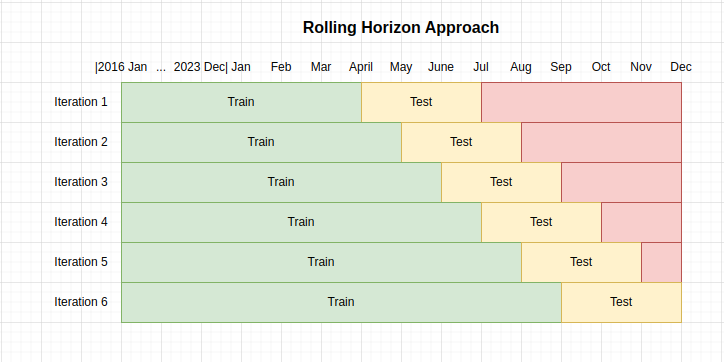
\includegraphics[width=0.5\linewidth]{figures/rha.png}
    \caption{Rolling Horizon Approach}
    \label{fig:rha} % Tag for referencing
\end{figure}

\subsection{ Analysis}

The performance of forecasting method is measured in terms of the relative error between predicted and actual values using Root-Mean-Squared-Percentage-Error (RMSPE)\cite{botchkarev_performance_2019}. Lower values in RMSPE indicate better performance. RMSPE measures the average percentage deviation between predicted and actual values, providing a standardized measure of prediction accuracy that is independent of the scale of the data. The data used for forecasting is not normalized and individual energy components have radically different scale. Hence, the RMSPE value provides better insight in evaluating forecasting models. RMSPE is defined as \\

\begin{equation}
\text{RMSPE} = \sqrt{\frac{1}{n} \sum_{i=1}^{n} \left( \frac{(Y_i - \hat{Y}_i)}{Y_i} \right)^2} \times 100
\end{equation}

\subsection{Data}

The dataset consists of monthly energy components contributing to the energy balance on the supply and demand side. The data are published by the national authorities of European countries (usually the transmission system operators or the national statistical offices) and are collected on the level of the high-voltage transmission grid. We use the time series on two different sampling frequency, one is the monthly value, while the other has the hourly resolution. The focus of this study is put on the key energy components or the components with the high level of variability, particularly electricity demand, and renewable energy generation such as wind, PV or hydro generation.  Electricity demand  is crucial for understanding how much power the system needs to meet consumer needs. Demand can vary significantly based on seasonal factors (heating/cooling), economic activity, and population growth. The increasing penetration of renewables significantly impacts supply dynamics. Understanding the variability of wind and solar generation, as well as the dispatchability (controllable generation) of hydro, is critical for managing grid integration challenges and optimizing renewable energy utilization. Data from the January of 2016 onwards is chosen as this period coincides with a significant ramp-up of renewable energy deployment across Europe. \\

\subsection{Infrastructure of the Framework}

As it can be seen in figure ~\ref{fig:framework}, the framework largely is capable of carrying out 2 tasks. One of them is forecasting a set of energy sources from a set of countries with designated models, and the other is producing a comprehensible visualization of a country's data or analysis of the forecasted data. \\ 

\begin{figure}[htp!]
    \centering
    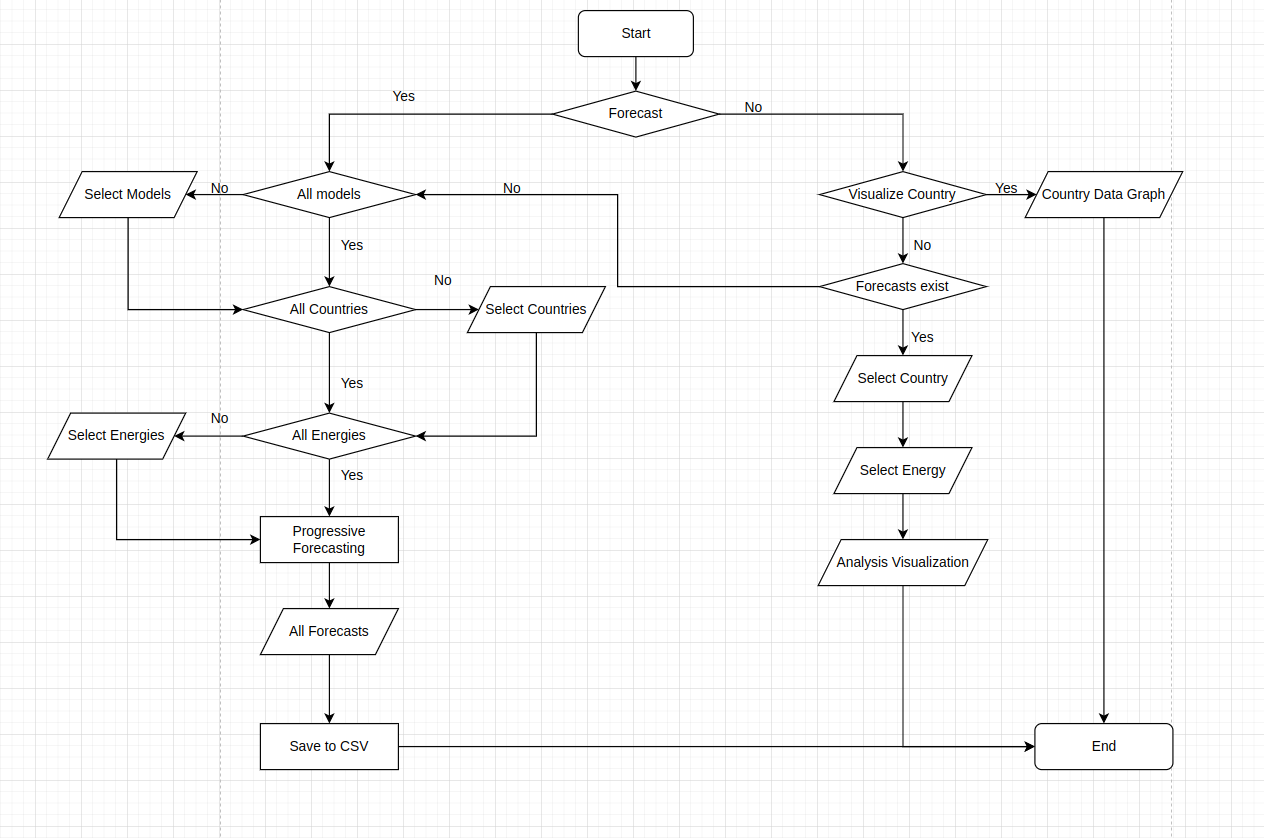
\includegraphics[width=0.5\linewidth]{figures/flowchart.png}
    \caption{Framework Flowchart}
    \label{fig:framework} % Tag for referencing
\end{figure}

\begin{itemize}
 \item Forecasting: When the user of the framework decides to forecast, they have to designate models to use, countries to look into, and energy sources they want to forecast. Then the collected data is passed to the function responsible for forecasting with rolling horizon approach, and the output data is saved as a CSV. Finally, the framework is terminated.\\
 \item Visualization: There are 2 options for visualization. The framework visualizes:
 \begin{itemize}
  \item specific energy data of a specific country along with the decomposition which indicates the trend, seasonality, and residual of the data.
  \item analysis of energy data forecast. The framework analyzes the forecasted data against the test data, and produces the analysis in terms of visual narratives to aid the viewer's understanding of all model's performance individually.\\
 \end{itemize}

 \end{itemize}
 
\section{Results \& Discussions}

\newpage

%%%%%
\bibliographystyle{abbrv}
\bibliography{references}

\end{document}
